\section{Applications of Linear Program}
\subsection{Game Theory}

\subsubsection{Two-Person Zero-Sum Games}

\begin{definition}[Zero-Sum Game, Payoff Matrix]
    We consider a game between players P1 and P2, where P1 has \(m\) actions labelled by \(\Bqty{1, 2, \ldots, m}\) and P2 has \(n\) actions labelled by \(\Bqty{1, 2, \ldots, n}\), where the \emph{payoff  matrix} \(\vb{A} = \pqty{a_{ij}} \in \RR^{m \times n}\) records the amount earned by P1 and lost by P2, if P1 plays \(i\) and \(P2\) plays \(j\).
\end{definition}

\begin{example}[Rock-Paper-Scissors]
    The payoff matrix given for the rock-paper-scissors game is given by
    \[
        \pqty{
            \begin{array}{c|ccc}
                & \text{R} & \text{P} & \text{S} \\
                \hline
                \text{R} & 0 & -1 & +1 \\
                \text{P} & +1 & 0 & -1 \\
                \text{S} & -1 & +1 & 0
            \end{array}
        }.
    \]
\end{example}

If P1 plays \(i\), then P1 should expect to have a payoff of
\[
    \min_{j \in \bqty{n}} a_{ij}
\]
since P2 would solve this optimisation problem for \(j\).

Hence, P1 will try to solve for \(i\) the problem
\[
    \max_{i \in \bqty{m}} \min_{j \in \bqty{n}} a_{ij},
\]
while P2 will try to solve for \(j\) the problem
\[
    \min_{j \in \bqty{n}} \max_{i \in \bqty{m}} a_{ij}.
\]

\subsubsection{Saddle Point and Value of Game}

\begin{example}[Saddle Point]
    Suppose
    \[
        \vb{A} = \pmqty{1 & 2 \\ 3 & 4}.
    \]

    Then P1 will decide to play \(i = 2\) (i.e., the second row, since its minimum is larger than the first, expecting \(j = 1\)), and P2 will decide to play \(j = 1\) (i.e., the first column, since its maximum is lower than the second, expecting \(i = 2\)). In this case, we happen to get
    \[
        \max_{i \in \bqty{m}} \min_{j \in \bqty{n}} a_{ij} = \min_{j \in \bqty{n}} \max_{i \in \bqty{m}} a_{ij} = 3
    \]
    so it does not matter which player plays first.
\end{example}

\begin{definition}[Saddle Point, Value of a Game]
    For a payoff matrix \(\vb{A}\), \(\pqty{i^{\ast}, j^{\ast}}\) is called a \emph{saddle point}, if it is both the minimum entry in row \(i^{\ast}\) and maximum entry in column \(j^{\ast}\). In this case,
    \[
        \max_{i \in \bqty{m}} \min_{j \in \bqty{n}} a_{ij} = \min_{j \in \bqty{n}} \max_{i \in \bqty{m}} a_{ij} = a_{i^{\ast}j^{\ast}}
    \]
    is called the \emph{value} of the game.
\end{definition}

If a saddle point exists, the order of playing does not matter.

\begin{example}[Non-Existence of Saddle Point]
    Consider the payoff matrix
    \[
        \vb{A} = \pmqty{4 & 2 \\ 1 & 3}.
    \]

    Then P1 will decide to play \(i = 2\) expecting \(j = 1\), while P2 will decide to play \(j = 2\) expecting \(i = 2\). These do not match, so there is no saddle point. Notice that in this case, the order of playing matters.
\end{example}

\subsubsection{Pure and Mixed Strategies}

\begin{definition}[Pure and Mixed Strategies]
    A \emph{pure} strategy for P1 is when they pick a fixed action \(i \in \bqty{m}\).

    A \emph{mixed} strategy P1 picks a probability distribution \(\vb{p}\) on their action
    \[
        \vb{p} = \begin{pmatrix}
            p_1 \\ p_2 \\ \vdots \\ p_m
        \end{pmatrix}.
    \]
\end{definition}

If P1 has mixed strategy \(\vb{p}\), the expected payoff is
\[
    \min_{j \in \bqty{n}} \sum_{i = 1}^{m} a_{ij} p_i,
\]
and therefore, now the optimisation problem becomes \emph{maximising} the quantity
\[
    \min_{j \in \bqty{n}} \sum_{i = 1}^{m} a_{ij} p_i
\]
subject to the constraints \(\vb{p} \geq \vb{0}\) and \(\sum_{i = 1}^{m} p_i = 1\).

This could be equivalently expressed as the linear program to \emph{maximise} \(v\), subject to
\[
    \vb{A}\transpose \vb{p} \geq v \vb{1}_n, \quad \vb{1}_m\transpose \vb{p} = 1 \qand \vb{p} \geq \vb{0},
\]
where we denote \(\vb{1}_{k} \in \RR^k\) to be the vector with all entries \(1\).

Similarly, we can write P2's optimisation problem as \emph{minimise} \(w\), subject to
\[
    \vb{A} \vb{q} \leq w \vb{1}_m, \quad \vb{1}_n\transpose \vb{q} = 1 \qand \vb{q} \geq \vb{0}.
\]

In fact, these two problems are duals of each other. Effectively, we found a saddle point `outside' of the matrix in a probability space, which is the point of \emph{Nash equilibrium}.

\begin{proposition}[Optimisation Problems for P1 and P2 are Duals]
    The optimisation problems for P1 and P2's mixed strategies are duals of each other.
\end{proposition}

\begin{proof}
    The Lagrangian of P2's problem is given by
    \begin{align*}
        L\pqty{w, \vb{q}, \vb{s}, \vb*{\lambda}_1, \lambda_2} &= w + \vb*{\lambda}_1\transpose \pqty{\vb{Aq} + \vb{s} - w \vb{1}_m} - \lambda_2 \pqty{\vb{1}_n\transpose \vb{q} - 1} \\
        &= w \pqty{1 - \vb*{\lambda}_1\transpose \vb{1}_m} + \pqty{\vb*{\lambda}_1\transpose \vb{A} - \lambda_2 \vb{1}_n\transpose} \vb{q} + \vb*{\lambda}_1\transpose \vb{s} + \lambda_2.
    \end{align*}

    The set
    \[
        \Lambda = \set{\vb*{\lambda} \in \RR^m}{
            \begin{aligned}
                \vb*{\lambda}_1\transpose \vb{1}_m &= 1 \\
                \vb*{\lambda}_1\transpose \vb{A} &\geq \lambda_2 \vb{1}_n\transpose \\
                \vb*{\lambda}_1 &\geq 0
            \end{aligned}}
    \]
    and we have if \(\vb*{\lambda_1} \in \Lambda\), then
    \[
        \min_{w, \vb{q}, \vb{s}} L = \lambda_2.
    \]

    Therefore, the dual problem is to maximise \(\lambda_2\), subject to the constraints stated in \(\Lambda\), which is precisely P1's optimisation problem, with \(\vb{p}\) as \(\vb*{\lambda}_1\), and \(v\) as \(\lambda_2\).
\end{proof}

\begin{theorem}[Optimal Strategies]
    A strategy \(\vb{p}\) is optimal for P1, if and only if there exists \(\vb{q}\) and \(v\), such that
    \begin{enumerate}
        \item Primal Feasibility: \(\vb{A}\transpose \vb{p} \geq v \vb{1}_n\), \(\vb{1}_m\transpose \vb{p} = 1\) and \(\vb{p} \geq \vb{0},\)
        \item Dual Feasibility: \(\vb{A} \vb{q} \leq w \vb{1}_m\), \(\vb{1}_n\transpose \vb{q} = 1\) and \(\vb{q} \geq \vb{0}.\)
        \item Complementary Slackness: \(v = \vb{p}\transpose \vb{Aq}\).
    \end{enumerate}
\end{theorem}

\begin{proof}
    It suffices to check the complementary slackness condition. If \(\pqty{\vb{p}, v}\) and \(\pqty{\vb{q}, w}\) are primal/dual optimal, then
    \[
        \pqty{\vb{Aq} - w \vb{1}_m}\transpose \vb{p} = 0 \qand \vb{q}\transpose \pqty{\vb{A}\transpose \vb{p} - v \vb{1}_n} = 0.
    \]

    Simplifying, we have
    \[
        w = v = \vb{p}\transpose \vb{A} \vb{q}
    \]
    as desired.
\end{proof}

\begin{example}[Rock-Paper-Scissors]
    In rock-paper-scissors, we have
    \[
        \vb{p} = \vb{q} = \begin{pmatrix}
            \flatfrac{1}{3} \\ \flatfrac{1}{3} \\ \flatfrac{1}{3}
        \end{pmatrix}
    \]
    with \(w = v = 0\).
\end{example}

\subsubsection{Finding Optimal Strategies}

Usually, we do not have to solve the whole linear program to find the optimal strategy -- some observations could be made to reduce the size of the matrix and the number of variables.

\begin{enumerate}
    \item Look for a saddle point in the matrix. If such saddle point exists, the optimal strategy is for both players to play at this saddle point.
    \item Look for dominating actions. Suppose for P1 that there exists \(i_1\) and \(i_2\), such that
    \[
        \forall j \in \bqty{n}: a_{i_1 j} \geq a_{i_2 j},
    \]
    then P1 would never play \(i_2\), so this action could be removed.

    Similarly, suppose for P2 that there exists \(j_1\) and \(j_2\), such that
    \[
        \forall i \in \bqty{m}: a_{i j_1} \leq a_{i j_2},
    \]
    then P2 would never play \(j_2\), so this action could be removed.
    \item Finally, we solve the linear program, which could be graphically, or of course, using the simplex method.
\end{enumerate}

\begin{example}
    Consider the payoff matrix
    \[
        \vb{A} = \pmqty{
            2 & 3 & 4 \\
            3 & 1 & \flatfrac{1}{2} \\
            1 & 3 & 2
        }.
    \]

    Notice that the first row dominates the third row, so P1 would never play action 3. This reduces to the new matrix
    \[
        \vb{A} = \pmqty{
            2 & 3 & 4 \\
            3 & 1 & \flatfrac{1}{2}
        }.
    \]

    Notice that currently there are no dominating columns, or saddle points. Now we solve for the linear program. Suppose
    \[
        \vb{p} = \pqty{p, 1 - p, 0}\transpose,
    \]
    then we want to maximise \(v\), subject to
    \[
        2p + 3 \pqty{1 - p} \geq v, \quad 3p + \pqty{1 - p} \geq v, \quad 4p + \frac{1 - p}{2} \geq v
    \]
    and
    \[
        0 \leq p \leq 1.
    \]

    The inequality constraints are equivalent to
    \[
        v \leq 3 - p, \quad v \leq 1 + 2p, \quad v \leq \flatfrac{1}{2} + \flatfrac{7p}{2}.
    \]

    Drawing these lines on the \(\pqty{p, v}\) plane, we get \autoref{fig:lp-graphic}, and we notice that \(v\) is maximised at the intersection of \(v = 1 + 2p\) and \(v = 3 - p\), which solves to \(p = \flatfrac{2}{3}\). This gives
    \[
        \vb{p} = \pqty{\flatfrac{2}{3}, \flatfrac{1}{3}, 0}\transpose
    \]
    and \(v = \flatfrac{7}{3}\).
    
    To solve for \(\vb{q}\), we use the complementary slackness equation. Notice that since the final constraint for \(p\) is not tight, we have \(q_3 = 0\), and hence setting \(\vb{q} = \pqty{q, 1 - q, 0}\), we have
    \[
        2q + 3 \pqty{1 - q} \leq w, \quad 3q + \pqty{1 - q} \leq w, \quad q + 3 \pqty{1 - q} \leq w.
    \]

    By complementary slackness, since \(p \neq 0\) and \(1 - q \neq 0\), the first two constraints must be tight, so we have
    \[
        3 - q = 2q + 1 = \frac{7}{3}
    \]
    and hence \(q = \flatfrac{2}{3}\), giving
    \[
        \vb{q} = \pqty{\flatfrac{2}{3}, \flatfrac{1}{3}, 0}.
    \]
\end{example}

\begin{figure}[ht!]
    \centering
    \begin{tikzpicture}
        \begin{axis}[
            width=10cm,
            height=7cm,
            axis lines=middle,
            xlabel={\(p\)},
            ylabel={\(v\)},
            xmin=-0.1, xmax=1.1,
            ymin=0, ymax=3.3,
            xtick={0,0.2,0.4,0.6,0.8,1},
            ytick={0,0.5,1,1.5,2,2.5,3},
            grid=both,
            legend pos=south east,
        ]

        % v = 3 - p
        \addplot[
            domain=-0.05:1.05,
            samples=2,
            thick
        ]{3-x};
        \addlegendentry{\(v = 3 - p\)}

        % v = 1 + 2p
        \addplot[
            domain=-0.05:1.05,
            samples=2,
            thick,
            dashed
        ]{1+2*x};
        \addlegendentry{\(v = 1 + 2p\)}

        % v = 1/2 + 7p/2
        \addplot[
            domain=-0.05:1.05,
            samples=2,
            thick,
            dotted
        ]{0.5+3.5*x};
        \addlegendentry{\(v = \flatfrac{1}{2}+ \flatfrac{7p}{2}\)}

        \end{axis}
    \end{tikzpicture}
    \caption{Linear Programming on the \(\pqty{p, v}\)-Plane}
    \label{fig:lp-graphic}%
\end{figure}

\subsection{Network Flow}

\begin{definition}[Directed and Undirected Graph, Vertices, Edges]
    A \emph{directed graph} \(G = \pqty{V, E}\) is a pair a set of \emph{vertices} \(V\), and a set of \emph{edges} \(E \subseteq V \times V\).

    If \(E\) is symmetric, then the graph is \emph{undirected graph}.
\end{definition}

\subsubsection{Minimum Cost Flow}

\begin{definition}[Flow, Source/Sink, Cost Matrix]
    Let \(G = \pqty{V, E}\) with \(\abs{V} = n\) labelled by \(1\) to \(n\). We assign a \emph{flow} \(x_{ij}\) for each edge \(\pqty{i, j} \in E\).

    We define a vector \(\vb{b} \in \RR^n\) (a function from \(V\) to \(\RR\)) as the amount of flow \(b_i\) that enters a vertex \(i\). If \(b_i > 0\), then vertex \(i\) is a \emph{source}; if \(b_i < 0\), then vertex \(i\) is a \emph{sink}. We always have \(\sum_{i = 1}^{n} b_i = 0\).

    We define a \emph{cost matrix} \(\vb{C} \in \RR^{n \times n}\) which is the cost per unit flow on the edge.

    We define matrices \(\underline{\vb{M}}, \overline{\vb{M}} \in \RR^{n \times n}\) to bound the costs \(\underline{m}_{ij} \leq x_{ij} \leq \overline{m}_{ij}\).
\end{definition}

\begin{definition}[Network Flow]
    The \emph{network flow} problem is to \emph{minimise} the total cost
    \[
        \sum_{\pqty{i, j} \in E} c_{ij} x_{ij}
    \]
    subject to the constraints:
    \begin{itemize}
        \item \emph{flow conservation} at a fixed vertex \(i \in V\)
        \[
            b_i + \sum_{j: \pqty{j, i} \in E} x_{ji} = \sum_{j: \pqty{i, j} \in E} x_{ij}
        \];
        \item the cost constraint \(\underline{m}_{ij} \leq c_{ij} \leq \overline{m}_{ij}\).
    \end{itemize}
\end{definition}

Notice that the requirement \(\sum_{i = 1}^{n} b_i = 0\) can be derived from flow conservation.

\subsubsection{The Transport Problem}

A special case of the network flow problem is the transport problem.

\begin{definition}[Suppilier, Consumer, Bipartite Graph]
    Suppose we have \(n\) \emph{suppliers} \(i \in \Bqty{1, 2, \ldots, n}\), each producing \(s_i\) amount of goods, and \(m\) consumers \emph{demand} \(j \in \Bqty{1, 2, \ldots, m}\), each demanding \(d_j\) amount of goods. We have
    \[
        \sum_{i = 1}^{n} s_i = \sum_{j = 1}^{m} d_j.
    \]

    The graph is a \emph{bipartite graph}, given by two sets of vertices, \(\bqty{n}\) and \(\bqty{m}\) (so in fact \(V\) is the \emph{disjoint} union of them), and with edges only within \(\bqty{n} \times \bqty{m}\). In this case, the cost matrix is defined as a \(n \times m\) matrix.
\end{definition}

\begin{definition}[Transport Problem]
    The \emph{transport problem} is to \emph{minimise} the total cost
    \[
        \sum_{i = 1}^{n} \sum_{j = 1}^{n} c_{ij} x_{ij}
    \]
    subject to the constraints
    \[
        \forall i \in \bqty{n}: \sum_{j = 1}^{m} x_{ij} = s_i
    \]
    and
    \[
        \forall j \in \bqty{m}: \sum_{i = 1}^{n} x_{ij} = d_j
    \]
    and
    \[
        \forall i \in \bqty{n}, j \in \bqty{m}: x_{ij} \geq 0
    \]  
\end{definition}

This is clearly a subset of network flow problem -- but in fact \emph{all} network flow problems (with certain requirements) can be converted into a transport problem!

\begin{theorem}[Network Flows can be recast as Transport Problems]
    \label{thm:network-flow-recast-transport}%
    Every minimum cost network flow problem with finite capacities (\(\overline{m}_{ij} < \plusinfty\)), or non-negative costs (\(c_{ij} \geq 0\)) can be recast as an equivalent transport problem.
\end{theorem}

\begin{remark}
    Given \(c_{ij} \geq 0\) for all \(i\) and \(j\), we could set
    \[
        \overline{m}_{ij} = \sum_{i \in V} \abs{b_i}
    \]
    if \(\overline{m}_{ij} = \plusinfty\).
\end{remark}

\begin{lemma}[Lower Bound could be Zero]
    For every network flow problem, the lower bound matrix \(\underline{\vb{M}}\) could, without loss of generality, be set to \(\vb{O}\), the zero matrix.
\end{lemma}

\begin{proof}
    Setting
    \[
        \tilde{x}_{ij} = x_{ij} - \underline{m}_{ij}
    \]
    changes the bounds to
    \[
        0 \leq \tilde{x}_{ij} \leq \overline{m}_{ij} - \underline{m}_{ij}.
    \]

    The new cost is therefore
    \[
        \sum c_{ij} \tilde{x}_{ij} = \sum c_{ij} x_{ij} - \sum c_{ij} \underline{m}_{ij}
    \]
    which is just differing by a constant.

    As for the flow condition, we substitute \(b_i\) by
    \[
        \tilde{b}_i = b_i + \sum_{j: \pqty{j, i} \in E} \underline{m}_{ji} - \sum_{j: \pqty{j, i} \in E} \underline{m}_{ij}
    \]
    which are, again, just changing by constants for fixed \(i\).
\end{proof}

\begin{proof}[Proof of \autoref{thm:network-flow-recast-transport}]
    We now construct a transport problem according to the minimum cost network flow problem, as demonstrated in \autoref{fig:transport-from-network-flow}.

    For every vertex \(i \in V\), we construct a consumer, which demands
    \[
        \sum_{k: \pqty{i, k} \in E} \overline{m}_{ik} - b_i.
    \]

    For every edge \(\pqty{i, j} \in E\), we construct a supplier, which produces \(\overline{m}_{ij}\) units.

    We set the costs to be
    \[
        c_{ij, i} = 0 \qand c_{ij, j} = c_{ij}.
    \]

    Let the flow from \(ij\) to \(j\) be \(x_{ij}\), and the (remaining) flow from \(ij\) to \(i\) be \(\overline{m}_{ij} - x_{ij}\). (This gives the transport conservation for the suppliers.)

    We notice that the total flow into consumer \(i\) is given by
    \[
        \sum_{k: \pqty{i, k} \in E} \pqty{\overline{m}_{ik} - x_{ik}} + \sum_{k: \pqty{k, i} \in E} x_{ki}
    \]
    and we want this to be equal to the demand at \(i\). This then gives the equality
    \[
        \sum_{k: \pqty{k, i} \in E} x_{ki} + b_i = \sum_{k: \pqty{i, k} \in E} x_{ik},
    \]
    giving the conservation of flow in the original network flow problem.

    For any solution \(x_{ij}\) to the transport problem, the cost is given by
    \[
        \sum_{\pqty{i, j} \in E} c_{ij} x_{ij}
    \]
    which gives identical costs.
\end{proof}

\begin{figure}[ht!]
    \centering
    \begin{tikzpicture}[
        scale=0.75,
        node distance=2cm,
        every node/.style={font=\Large},
        vertex/.style={
            circle,
            draw,
            minimum size=1.15cm,
            inner sep=0pt
        }
    ]

        \node[vertex] (ij) at (0, 0) {\(\pqty{i,j}\)};
        \node[vertex] (i) at (5, 5) {\(i\)};
        \node[vertex] (j) at (5, -5) {\(j\)};

        \draw[<-] (ij) -- ++(-3, 0)
            node[left] {\(\overline{m}_{ij}\)};

        \draw[->] (ij) -- (i)
            node[midway, above left] {\(c_{ij, i} = 0\)}
            node[midway, below right] {\(x_{ij, i} = \overline{m}_{ij} - x_{ij}\)};
        \draw[->] (ij) -- (j)
            node[midway, below left] {\(c_{ij, j} = c_{ij}\)}
            node[midway, above right] {\(x_{ij, j} = x_{ij}\)};

        \draw[->] (i) -- ++(3,0)
            node[right] {\(\displaystyle \sum_{k: \pqty{i, k} \in E} \overline{m}_{ik} - b_i\)};
        \draw[->] (j) -- ++(3,0)
            node[right] {\(\displaystyle \sum_{k: \pqty{j, k} \in E} \overline{m}_{jk} - b_j\)};

    \end{tikzpicture}
    \caption{Construction of Transport Problem from Network Flow}
    \label{fig:transport-from-network-flow}%
\end{figure}

\subsubsection{The Transport Algorithm}

\paragraph{Optimality Conditions}

The following optimality conditions for the transport problem arises from that for linear programs.

\begin{theorem}[Optimality Conditions for Transport Problem]
    If, for some feasible \(\pqty{x_{ij}}\), and we have dual variables \(\vb*{\lambda} \in \RR^n\), \(\vb*{\mu} \in \RR^m\) such that for all \(i \in \bqty{n}\) and \(j \in \bqty{m}\), we have
    \[
        c_{ij} \geq \lambda_i + \mu_j
    \]
    and
    \[
        \pqty{c_{ij} - \pqty{\lambda_i + \mu_j}} x_{ij} = 0
    \]
    then \(\pqty{x_{ij}}\) is optimal.
\end{theorem}

\begin{proof}
    The Lagrangian is given by
    \begin{align*}
        L\pqty{\pqty{x_{ij}}, \vb*{\lambda}, \vb*{\mu}} &= \sum_{i = 1}^{n} \sum_{j = 1}^{m} c_{ij} x_{ij} - \sum_{i = 1}^{n} \lambda_i \pqty{\sum_{j = 1}^{m} x_{ij} - s_i} - \sum_{j = 1}^{m} \mu_j \pqty{\sum_{i = 1}^{n} x_{ij} - d_j} \\
        &= \sum_{i = 1}^{n} \sum_{j = 1}^{m} \pqty{c_{ij} - \lambda_i - \mu_j} x_{ij} + \sum_{i = 1}^{n} \lambda_i s_i + \sum_{j = 1}^{m} \mu_j d_j.
    \end{align*}

    Dual feasibility is guaranteed by \(c_{ij} - \lambda_i - \mu_j \geq 0\), i.e. \(c_{ij} \geq \lambda_i + \mu_j\). The second condition gives complementary slackness. Using \autoref{thm:optimality-condition-lp} (Optimality Conditions for Linear Programs), we may conclude \(\pqty{x_{ij}}\) is optimal.
\end{proof}

\begin{remark}
    For a given basic feasible solution \(\pqty{x_{ij}}\), when we attempt to solve for \(\pqty{\vb*{\lambda}, \vb*{\mu}}\) using complementary slackness, we may assume \(\lambda_1 = 0\) without loss of generality -- since all equations assert the values of \(\lambda_i + \mu_j\).
\end{remark}

\paragraph{The Simplex Tableau}

To solve the transport problem efficiently, we use the \emph{transport tableau} which takes the form as in \autoref{tab:transport-tableau}.

\begin{table}[ht!]
    \centering
    \[
        \renewcommand{\arraystretch}{1.5}
        \begin{array}{c
            !{\vrule width 1.2pt}
            cc|cc|cc|cc|c}

            \multicolumn{1}{c}{} &
            \multicolumn{2}{c}{\mu_1} &
            \multicolumn{2}{c}{\mu_2} &
            \multicolumn{2}{c}{\cdots} &
            \multicolumn{2}{c}{\mu_m} &
            \\

            \noalign{\global\arrayrulewidth=1.2pt}
            \cline{2-9}
            \noalign{\global\arrayrulewidth=0.4pt}

            \multirow{2}{*}{\(\lambda_1\)}
            &
            \multicolumn{2}{c|}{\lambda_1+\mu_1} &
            \multicolumn{2}{c|}{\lambda_1+\mu_2} &
            \multicolumn{2}{c|}{\cdots} &
            \multicolumn{2}{c!{\vrule width 1.2pt}}{\lambda_1+\mu_m} &
            \multirow{2}{*}{\(s_1\)}
            \\

            \cline{3-3}
            \cline{5-5}
            \cline{7-7}
            \cline{9-9}

            &
            x_{11} & \multicolumn{1}{|c|}{c_{11}} &
            x_{12} & \multicolumn{1}{|c|}{c_{12}} &
            \cdots & \multicolumn{1}{|c|}{\cdots} &
            x_{1m} & \multicolumn{1}{|c!{\vrule width 1.2pt}}{c_{1m}} &
            \\

            \cline{2-9}

            \multirow{2}{*}{\(\lambda_2\)}
            &
            \multicolumn{2}{c|}{\lambda_2+\mu_1} &
            \multicolumn{2}{c|}{\lambda_2+\mu_2} &
            \multicolumn{2}{c|}{\cdots} &
            \multicolumn{2}{c!{\vrule width 1.2pt}}{\lambda_2+\mu_m} &
            \multirow{2}{*}{\(s_2\)}
            \\

            \cline{3-3}
            \cline{5-5}
            \cline{7-7}
            \cline{9-9}

            &
            x_{21} & \multicolumn{1}{|c|}{c_{21}} &
            x_{22} & \multicolumn{1}{|c|}{c_{22}} &
            \cdots & \multicolumn{1}{|c|}{\cdots} &
            x_{2m} & \multicolumn{1}{|c!{\vrule width 1.2pt}}{c_{2m}} &
            \\

            \cline{2-9}

            \multirow{2}{*}{\vdots}
            &
            \multicolumn{2}{c|}{\cdots} &
            \multicolumn{2}{c|}{\cdots} &
            \multicolumn{2}{c|}{\cdots} &
            \multicolumn{2}{c!{\vrule width 1.2pt}}{\cdots} &
            \multirow{2}{*}{\vdots}
            \\

            \cline{3-3}
            \cline{5-5}
            \cline{7-7}
            \cline{9-9}

            &
            \cdots & \multicolumn{1}{|c|}{\cdots} &
            \cdots & \multicolumn{1}{|c|}{\cdots} &
            \cdots & \multicolumn{1}{|c|}{\cdots} &
            \cdots & \multicolumn{1}{|c!{\vrule width 1.2pt}}{\cdots} &
            \\

            \cline{2-9}

            \multirow{2}{*}{\(\lambda_n\)}
            &
            \multicolumn{2}{c|}{\lambda_n+\mu_1} &
            \multicolumn{2}{c|}{\lambda_n+\mu_2} &
            \multicolumn{2}{c|}{\cdots} &
            \multicolumn{2}{c!{\vrule width 1.2pt}}{\lambda_n+\mu_m} &
            \multirow{2}{*}{\(s_n\)}
            \\

            \cline{3-3}
            \cline{5-5}
            \cline{7-7}
            \cline{9-9}
            &
            x_{n1} & \multicolumn{1}{|c|}{c_{n1}} &
            x_{n2} & \multicolumn{1}{|c|}{c_{n2}} &
            \cdots & \multicolumn{1}{|c|}{\cdots} &
            x_{nm} & \multicolumn{1}{|c!{\vrule width 1.2pt}}{c_{nm}} &
            \\

            \noalign{\global\arrayrulewidth=1.2pt}
            \cline{2-9}
            \noalign{\global\arrayrulewidth=0.4pt}

            \multicolumn{1}{c}{} &
            \multicolumn{2}{c}{d_1} &
            \multicolumn{2}{c}{d_2} &
            \multicolumn{2}{c}{\cdots} &
            \multicolumn{2}{c}{d_m} &

        \end{array}
        \renewcommand{\arraystretch}{1}
    \]
    \caption{Transport Tableau}
    \label{tab:transport-tableau}%
\end{table}

Note that \(d_j\), \(s_i\) and \(c_{ij}\) are defined by the problem, and \emph{not} updated during the algorithm.

\paragraph{The North-West Corner Rule}

The north-west corner rule is a way to find a feasible solution to the transport problem. It is completed by attempting to satisfy the supply/demand of consumers, starting from the top to the bottom.

\begin{algorithm}[ht!]
    \caption{North-West Corner Rule}\label{alg:north-west-corner-rule}%
    \begin{algorithmic}
        \Function{NorthWestCornerRule}{\(\vb{s} \in \RR^n, \vb{d} 
        \in \RR^m\)}
            \State \(i \gets 1\)
            \State \(j \gets 1\)

            \Statex

            \While{\(i \leq n\) \textbf{and} \(j \leq m\)}
                \LComment{Assign the maximum possible flow to use up either the remaining supply or demand}

                \State \(x_{ij} \gets \min \Bqty{s_i, d_j}\)
                \State \(s_i \gets s_i - x_{ij}\)
                \State \(d_j \gets d_j - x_{ij}\)

                \Statex 

                \LComment{At least one of the following ifs are executed}
                
                \If{\(s_i = 0\)}
                    \State \(i \gets i + 1\)
                \EndIf

                \If{\(d_j = 0\)}
                    \State \(j \gets j + 1\)
                \EndIf
            \EndWhile

            \State \Return{\(\pqty{x_{ij}}\)}
        \EndFunction
    \end{algorithmic}
\end{algorithm}

\paragraph{The Transport Algorithm} The \emph{transport algorithm} works as follows:
\begin{enumerate}
    \item If \(c_{ij} \geq \lambda_i + \mu_j\) for all \(\pqty{i, j}\), then the current solution is optimal and the algorithm stops.
    \item If \(c_{ij} < \lambda_i + \mu_j\) for some \(\pqty{i, j}\), then select that edge and find edges in the current flow that forms a cycle with it.
    \item Increase the flow in the new edge \(x_{ij}\), until some flow in the cycle reaches zero.
    \item Re-calculate the dual variables and repeat this process.
\end{enumerate}

\begin{example}[Transport Problem]
    \label{ex:transposrt-problem}%
    Suppose we have a transport problem defined by
    \[
        \vb{s} = \pqty{14, 10, 9}\transpose \qand \vb{d} = \pqty{12, 5, 8, 8}\transpose
    \]
    and the cost matrix
    \[
        \vb{C} = \pmqty{
            5 & 3 & 4 & 6 \\
            2 & 7 & 4 & 1 \\
            5 & 6 & 2 & 4
        }.
    \]

    By applying \autoref{alg:north-west-corner-rule}, we arrive at a feasible solution
    \begin{center}
        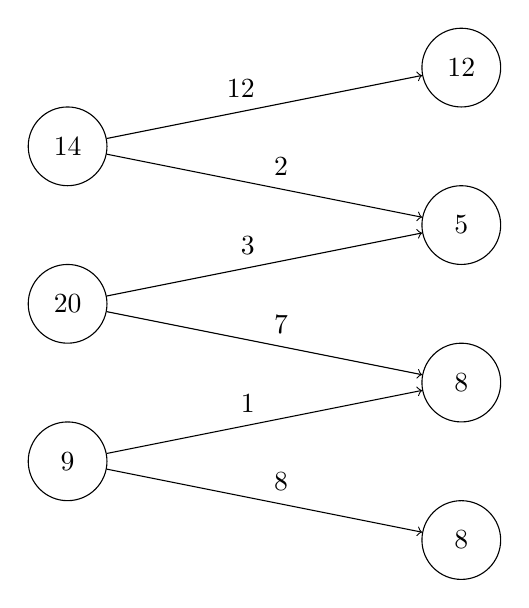
\begin{tikzpicture}[
            node distance=2cm,
            vertex/.style={
                circle,
                draw,
                minimum size=1cm,
                inner sep=0pt
            }
        ]

            \node[vertex] (s1) at (0, 2) {\(14\)};
            \node[vertex] (s2) at (0, 0) {\(20\)};
            \node[vertex] (s3) at (0, -2) {\(9\)};


            \node[vertex] (d1) at (5, 3) {\(12\)};
            \node[vertex] (d2) at (5, 1) {\(5\)};
            \node[vertex] (d3) at (5, -1) {\(8\)};
            \node[vertex] (d4) at (5, -3) {\(8\)};

            \draw[->] (s1) -- (d1)
                node[midway, above left] {\(12\)};
            \draw[->] (s1) -- (d2)
                node[midway, above right] {\(2\)};

            \draw[->] (s2) -- (d2)
                node[midway, above left] {\(3\)};
            \draw[->] (s2) -- (d3)
                node[midway, above right] {\(7\)};

            \draw[->] (s3) -- (d3)
                node[midway, above left] {\(1\)};
            \draw[->] (s3) -- (d4)
                node[midway, above right] {\(8\)};

        \end{tikzpicture}
    \end{center}
    with the flow matrix
    \[
        \pqty{x_{ij}} = \pmqty{
            12 & 2 & 0 & 0 \\
            0 & 3 & 7 & 0 \\
            0 & 0 & 1 & 8
        }.
    \]

    We now calculate the dual variables. By complementary slackness, we must have
    \begin{align*}
        \lambda_1 + \mu_1 = 5, & \quad \lambda_1 + \mu_2 = 3, \\
        \lambda_2 + \mu_2 = 7, & \quad \lambda_2 + \mu_3 = 4, \\
        \lambda_3 + \mu_3 = 2, & \quad \lambda_3 + \mu_4 = 4.
    \end{align*}

    Setting \(\lambda_1 = 0\), we solve to get
    \[
        \vb*{\lambda} = \pqty{0, 4, 2}\transpose \qand \vb*{\mu} = \pqty{5, 3, 0, 2}\transpose
    \]

    We can put this into a transport tableau:
    \[
        \renewcommand{\arraystretch}{1.5}
        \begin{array}{c
            !{\vrule width 1.2pt}
            cc|cc|cc|cc|c}

            \multicolumn{1}{c}{} &
            \multicolumn{2}{c}{5} &
            \multicolumn{2}{c}{3} &
            \multicolumn{2}{c}{0} &
            \multicolumn{2}{c}{2} &
            \\

            \noalign{\global\arrayrulewidth=1.2pt}
            \cline{2-9}
            \noalign{\global\arrayrulewidth=0.4pt}

            \multirow{2}{*}{\(0\)}
            &
            \multicolumn{2}{c|}{5} &
            \multicolumn{2}{c|}{3} &
            \multicolumn{2}{c|}{0} &
            \multicolumn{2}{c!{\vrule width 1.2pt}}{2} &
            \multirow{2}{*}{\(14\)}
            \\

            \cline{3-3}
            \cline{5-5}
            \cline{7-7}
            \cline{9-9}

            &
            12 & \multicolumn{1}{|c|}{5} &
            2  & \multicolumn{1}{|c|}{3} &
            0  & \multicolumn{1}{|c|}{4} &
            0  & \multicolumn{1}{|c!{\vrule width 1.2pt}}{6} &
            \\

            \cline{2-9}

            \multirow{2}{*}{\(4\)}
            &
            \multicolumn{2}{c|}{\boxed{9^{\ast}}} &
            \multicolumn{2}{c|}{7} &
            \multicolumn{2}{c|}{4} &
            \multicolumn{2}{c!{\vrule width 1.2pt}}{\boxed{6}} &
            \multirow{2}{*}{\(10\)}
            \\

            \cline{3-3}
            \cline{5-5}
            \cline{7-7}
            \cline{9-9}

            &
            0 & \multicolumn{1}{|c|}{2} &
            3 & \multicolumn{1}{|c|}{7} &
            7 & \multicolumn{1}{|c|}{4} &
            0 & \multicolumn{1}{|c!{\vrule width 1.2pt}}{1} &
            \\

            \cline{2-9}

            \multirow{2}{*}{\(2\)}
            &
            \multicolumn{2}{c|}{\boxed{7}} &
            \multicolumn{2}{c|}{5} &
            \multicolumn{2}{c|}{2} &
            \multicolumn{2}{c!{\vrule width 1.2pt}}{4} &
            \multirow{2}{*}{\(9\)}
            \\

            \cline{3-3}
            \cline{5-5}
            \cline{7-7}
            \cline{9-9}

            &
            0 & \multicolumn{1}{|c|}{5} &
            0 & \multicolumn{1}{|c|}{6} &
            1 & \multicolumn{1}{|c|}{2} &
            8 & \multicolumn{1}{|c!{\vrule width 1.2pt}}{4} &
            \\

            \noalign{\global\arrayrulewidth=1.2pt}
            \cline{2-9}
            \noalign{\global\arrayrulewidth=0.4pt}

            \multicolumn{1}{c}{} &
            \multicolumn{2}{c}{12} &
            \multicolumn{2}{c}{5} &
            \multicolumn{2}{c}{8} &
            \multicolumn{2}{c}{8} &

        \end{array}
        \renewcommand{\arraystretch}{1}
    \]

    Observe that the boxed entries do not satisfy the optimality conditions. Looking at the \(9, 0, 2\) entry, using ideas from the simplex algorithm, this means we need to add an edge from the second supplier to the first consumer, and push as much flow onto it as possible. Say the weight reassigned onto this new edge is \(\theta\).

    \begin{center}
        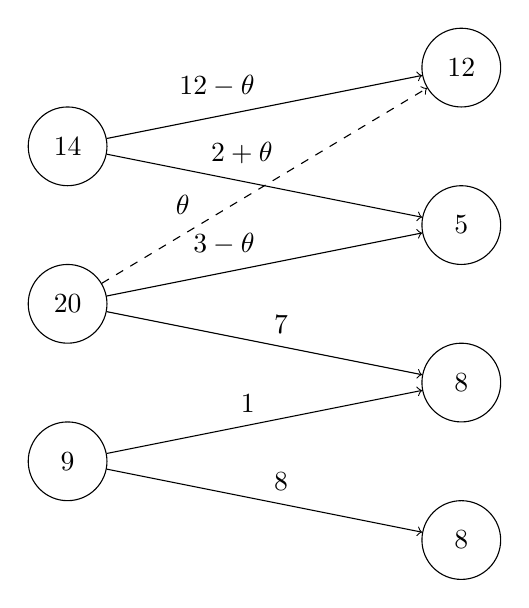
\begin{tikzpicture}[
            node distance=2cm,
            vertex/.style={
                circle,
                draw,
                minimum size=1cm,
                inner sep=0pt
            }
        ]

            \node[vertex] (s1) at (0, 2) {\(14\)};
            \node[vertex] (s2) at (0, 0) {\(20\)};
            \node[vertex] (s3) at (0, -2) {\(9\)};


            \node[vertex] (d1) at (5, 3) {\(12\)};
            \node[vertex] (d2) at (5, 1) {\(5\)};
            \node[vertex] (d3) at (5, -1) {\(8\)};
            \node[vertex] (d4) at (5, -3) {\(8\)};

            \draw[->] (s1) -- (d1)
                node[midway, above left] {\(12 - \theta\)};
            \draw[->] (s1) -- (d2)
                node[pos=0.3, above right] {\(2 + \theta\)};

            \draw[->, dashed] (s2) -- (d1)
                node[pos=0.3, above left] {\(\theta\)};

            \draw[->] (s2) -- (d2)
                node[midway, above left] {\(3 - \theta\)};
            \draw[->] (s2) -- (d3)
                node[midway, above right] {\(7\)};

            \draw[->] (s3) -- (d3)
                node[midway, above left] {\(1\)};
            \draw[->] (s3) -- (d4)
                node[midway, above right] {\(8\)};

        \end{tikzpicture}
    \end{center}

    Set \(\theta = 3\) since any \(\theta\) greater than this would mean a negative flow. This gives the new flow diagram
    \begin{center}
        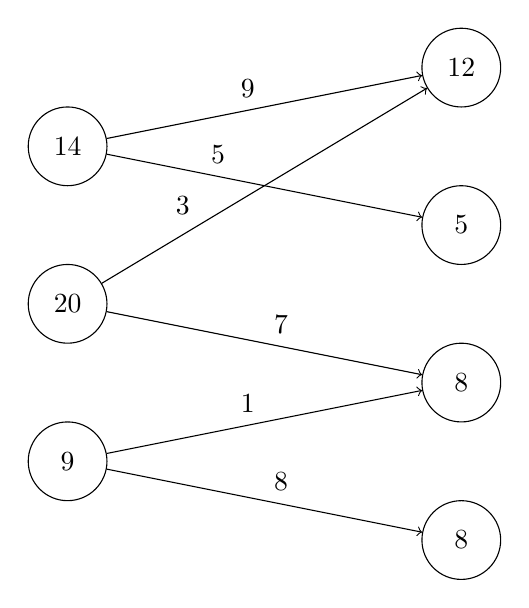
\begin{tikzpicture}[
            node distance=2cm,
            vertex/.style={
                circle,
                draw,
                minimum size=1cm,
                inner sep=0pt
            }
        ]

            \node[vertex] (s1) at (0, 2) {\(14\)};
            \node[vertex] (s2) at (0, 0) {\(20\)};
            \node[vertex] (s3) at (0, -2) {\(9\)};


            \node[vertex] (d1) at (5, 3) {\(12\)};
            \node[vertex] (d2) at (5, 1) {\(5\)};
            \node[vertex] (d3) at (5, -1) {\(8\)};
            \node[vertex] (d4) at (5, -3) {\(8\)};

            \draw[->] (s1) -- (d1)
                node[midway, above left] {\(9\)};
            \draw[->] (s1) -- (d2)
                node[pos=0.3, above right] {\(5\)};

            \draw[->] (s2) -- (d1)
                node[pos=0.3, above left] {\(3\)};
            \draw[->] (s2) -- (d3)
                node[midway, above right] {\(7\)};

            \draw[->] (s3) -- (d3)
                node[midway, above left] {\(1\)};
            \draw[->] (s3) -- (d4)
                node[midway, above right] {\(8\)};

        \end{tikzpicture}
    \end{center}
    with the transport tableau
    \[
        \renewcommand{\arraystretch}{1.5}
        \begin{array}{c
            !{\vrule width 1.2pt}
            cc|cc|cc|cc|c}

            \multicolumn{1}{c}{} &
            \multicolumn{2}{c}{5} &
            \multicolumn{2}{c}{3} &
            \multicolumn{2}{c}{7} &
            \multicolumn{2}{c}{9} &
            \\

            \noalign{\global\arrayrulewidth=1.2pt}
            \cline{2-9}
            \noalign{\global\arrayrulewidth=0.4pt}

            \multirow{2}{*}{\(0\)}
            &
            \multicolumn{2}{c|}{5} &
            \multicolumn{2}{c|}{3} &
            \multicolumn{2}{c|}{\boxed{7}} &
            \multicolumn{2}{c!{\vrule width 1.2pt}}{\boxed{9}} &
            \multirow{2}{*}{\(14\)}
            \\

            \cline{3-3}
            \cline{5-5}
            \cline{7-7}
            \cline{9-9}

            &
            9 & \multicolumn{1}{|c|}{5} &
            5  & \multicolumn{1}{|c|}{3} &
            0  & \multicolumn{1}{|c|}{4} &
            0  & \multicolumn{1}{|c!{\vrule width 1.2pt}}{6} &
            \\

            \cline{2-9}

            \multirow{2}{*}{\(-3\)}
            &
            \multicolumn{2}{c|}{2} &
            \multicolumn{2}{c|}{3} &
            \multicolumn{2}{c|}{4} &
            \multicolumn{2}{c!{\vrule width 1.2pt}}{\boxed{6^{\ast}}} &
            \multirow{2}{*}{\(10\)}
            \\

            \cline{3-3}
            \cline{5-5}
            \cline{7-7}
            \cline{9-9}

            &
            3 & \multicolumn{1}{|c|}{2} &
            0 & \multicolumn{1}{|c|}{7} &
            7 & \multicolumn{1}{|c|}{4} &
            0 & \multicolumn{1}{|c!{\vrule width 1.2pt}}{1} &
            \\

            \cline{2-9}

            \multirow{2}{*}{\(-5\)}
            &
            \multicolumn{2}{c|}{0} &
            \multicolumn{2}{c|}{-2} &
            \multicolumn{2}{c|}{2} &
            \multicolumn{2}{c!{\vrule width 1.2pt}}{4} &
            \multirow{2}{*}{\(9\)}
            \\

            \cline{3-3}
            \cline{5-5}
            \cline{7-7}
            \cline{9-9}

            &
            0 & \multicolumn{1}{|c|}{5} &
            0 & \multicolumn{1}{|c|}{6} &
            1 & \multicolumn{1}{|c|}{2} &
            8 & \multicolumn{1}{|c!{\vrule width 1.2pt}}{4} &
            \\

            \noalign{\global\arrayrulewidth=1.2pt}
            \cline{2-9}
            \noalign{\global\arrayrulewidth=0.4pt}

            \multicolumn{1}{c}{} &
            \multicolumn{2}{c}{12} &
            \multicolumn{2}{c}{5} &
            \multicolumn{2}{c}{8} &
            \multicolumn{2}{c}{8} &

        \end{array}
        \renewcommand{\arraystretch}{1}
    \]

    We now deal with the \(6, 0, 1\) entry. This adds the new edge
    \begin{center}
        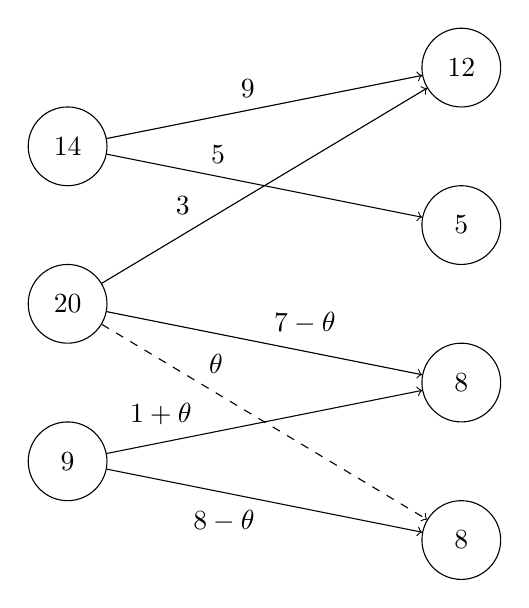
\begin{tikzpicture}[
            node distance=2cm,
            vertex/.style={
                circle,
                draw,
                minimum size=1cm,
                inner sep=0pt
            }
        ]

            \node[vertex] (s1) at (0, 2) {\(14\)};
            \node[vertex] (s2) at (0, 0) {\(20\)};
            \node[vertex] (s3) at (0, -2) {\(9\)};


            \node[vertex] (d1) at (5, 3) {\(12\)};
            \node[vertex] (d2) at (5, 1) {\(5\)};
            \node[vertex] (d3) at (5, -1) {\(8\)};
            \node[vertex] (d4) at (5, -3) {\(8\)};

            \draw[->] (s1) -- (d1)
                node[midway, above left] {\(9\)};
            \draw[->] (s1) -- (d2)
                node[pos=0.3, above right] {\(5\)};

            \draw[->] (s2) -- (d1)
                node[pos=0.3, above left] {\(3\)};
            \draw[->] (s2) -- (d3)
                node[midway, above right] {\(7 - \theta\)};

            \draw[->] (s3) -- (d3)
                node[pos=0.3, above left] {\(1 + \theta\)};
            \draw[->] (s3) -- (d4)
                node[midway, below left] {\(8 - \theta\)};

            \draw[->, dashed] (s2) -- (d4)
                node[pos=0.3, above right] {\(\theta\)};

        \end{tikzpicture}
    \end{center}
    and we maximise to get \(\theta = 7\), giving the new flow diagram
        \begin{center}
        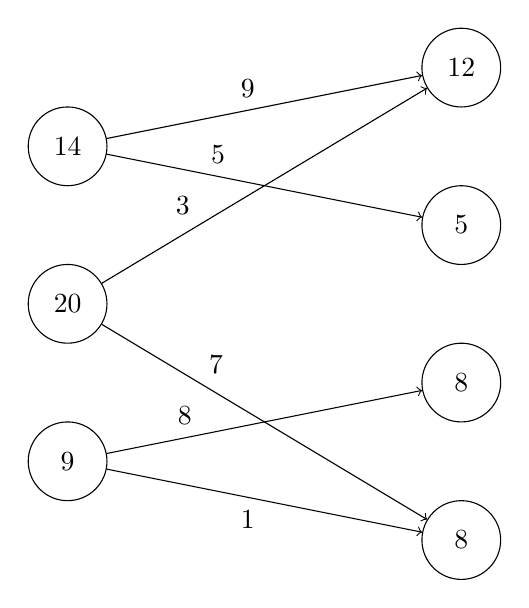
\begin{tikzpicture}[
            node distance=2cm,
            vertex/.style={
                circle,
                draw,
                minimum size=1cm,
                inner sep=0pt
            }
        ]

            \node[vertex] (s1) at (0, 2) {\(14\)};
            \node[vertex] (s2) at (0, 0) {\(20\)};
            \node[vertex] (s3) at (0, -2) {\(9\)};


            \node[vertex] (d1) at (5, 3) {\(12\)};
            \node[vertex] (d2) at (5, 1) {\(5\)};
            \node[vertex] (d3) at (5, -1) {\(8\)};
            \node[vertex] (d4) at (5, -3) {\(8\)};

            \draw[->] (s1) -- (d1)
                node[midway, above left] {\(9\)};
            \draw[->] (s1) -- (d2)
                node[pos=0.3, above right] {\(5\)};

            \draw[->] (s2) -- (d1)
                node[pos=0.3, above left] {\(3\)};

            \draw[->] (s3) -- (d3)
                node[pos=0.3, above left] {\(8\)};
            \draw[->] (s3) -- (d4)
                node[midway, below left] {\(1\)};

            \draw[->] (s2) -- (d4)
                node[pos=0.3, above right] {\(7\)};

        \end{tikzpicture}
    \end{center}
    and transport tableau
    \[
        \renewcommand{\arraystretch}{1.5}
        \begin{array}{c
            !{\vrule width 1.2pt}
            cc|cc|cc|cc|c}

            \multicolumn{1}{c}{} &
            \multicolumn{2}{c}{5} &
            \multicolumn{2}{c}{3} &
            \multicolumn{2}{c}{2} &
            \multicolumn{2}{c}{4} &
            \\

            \noalign{\global\arrayrulewidth=1.2pt}
            \cline{2-9}
            \noalign{\global\arrayrulewidth=0.4pt}

            \multirow{2}{*}{\(0\)}
            &
            \multicolumn{2}{c|}{5} &
            \multicolumn{2}{c|}{3} &
            \multicolumn{2}{c|}{2} &
            \multicolumn{2}{c!{\vrule width 1.2pt}}{4} &
            \multirow{2}{*}{\(14\)}
            \\

            \cline{3-3}
            \cline{5-5}
            \cline{7-7}
            \cline{9-9}

            &
            9 & \multicolumn{1}{|c|}{5} &
            5  & \multicolumn{1}{|c|}{3} &
            0  & \multicolumn{1}{|c|}{4} &
            0  & \multicolumn{1}{|c!{\vrule width 1.2pt}}{6} &
            \\

            \cline{2-9}

            \multirow{2}{*}{\(-3\)}
            &
            \multicolumn{2}{c|}{2} &
            \multicolumn{2}{c|}{0} &
            \multicolumn{2}{c|}{-1} &
            \multicolumn{2}{c!{\vrule width 1.2pt}}{1} &
            \multirow{2}{*}{\(10\)}
            \\

            \cline{3-3}
            \cline{5-5}
            \cline{7-7}
            \cline{9-9}

            &
            3 & \multicolumn{1}{|c|}{2} &
            0 & \multicolumn{1}{|c|}{7} &
            0 & \multicolumn{1}{|c|}{4} &
            7 & \multicolumn{1}{|c!{\vrule width 1.2pt}}{1} &
            \\

            \cline{2-9}

            \multirow{2}{*}{\(0\)}
            &
            \multicolumn{2}{c|}{5} &
            \multicolumn{2}{c|}{3} &
            \multicolumn{2}{c|}{2} &
            \multicolumn{2}{c!{\vrule width 1.2pt}}{4} &
            \multirow{2}{*}{\(9\)}
            \\

            \cline{3-3}
            \cline{5-5}
            \cline{7-7}
            \cline{9-9}

            &
            0 & \multicolumn{1}{|c|}{5} &
            0 & \multicolumn{1}{|c|}{6} &
            8 & \multicolumn{1}{|c|}{2} &
            1 & \multicolumn{1}{|c!{\vrule width 1.2pt}}{4} &
            \\

            \noalign{\global\arrayrulewidth=1.2pt}
            \cline{2-9}
            \noalign{\global\arrayrulewidth=0.4pt}

            \multicolumn{1}{c}{} &
            \multicolumn{2}{c}{12} &
            \multicolumn{2}{c}{5} &
            \multicolumn{2}{c}{8} &
            \multicolumn{2}{c}{8} &

        \end{array}
        \renewcommand{\arraystretch}{1}
    \]

    This satisfies the optimality conditions, hence solves the problem.
\end{example}

\subsection{Maximum Flow and Minimum Cut}
\subsubsection{Maximum Flow}

We now consider a directed graph with \emph{capacities} assigned to each edges. We want to maximise the flow from the source to the sink by assigning flows along each edge, while not exceeding the capacities of each edge. (Of course, the flow conservation equation must be satisfied). Without loss of generality, assume the source vertex is \(1\) and the sink vertex is \(n\).

\begin{definition}[Maximum Flow Problem]
    For a graph \(G = \pqty{V, E}\) and a matrix \(c_{ij}\) defined on its edges (the capacities of each edge), the \emph{maximum flow problem} is to \emph{maximise} \(\delta\), the flow, subject to constraints
    \begin{itemize}
        \item \emph{outgoing flow} from vertex \(1\):
        \[
            \sum_{j: \pqty{1, j} \in E} x_{1j} - \sum_{i: \pqty{i, 1} \in E} x_{i1} = \delta;
        \]
        \item \emph{incoming flow} to vertex \(n\):
        \[
            \sum_{i: \pqty{i, n} \in E} x_{in} - \sum_{j: \pqty{n, j} \in E} x_{nj} = \delta;
        \]
        \item \emph{flow conservation} at vertex \(i \neq 1, n\):
        \[
            \sum_{j: \pqty{i, j} \in E} x_{ij} = \sum_{j: \pqty{j, i} \in E} x_{ji};
        \]
        \item \emph{capacity constraint}: for all \(\pqty{i, j} \in E\),
        \[
            0 \leq x_{ij} \leq c_{ij}.
        \]
    \end{itemize}
\end{definition}

\begin{notation}
    Introducing the notation for the net amount of flow leaving a node
    \[
        \phi_i \pqty{x} = \sum_{j: \pqty{i, j} \in E} x_{ij} - \sum_{j: \pqty{j, i} \in E} x_{ji}
    \]
    and an indicator
    \[
        b_i = \begin{cases}
            +1, &\qif i = 1, \\
            -1, &\qif i = n, \\
            0, &\qotherwise.
        \end{cases}
    \]
    then the problem became maximising \(\delta\), subject to constraints
    \[
        \phi_i \pqty{x} - b_i \delta = 0
    \]
    for all \(i\), and \(0 \leq x_{ij} \leq c_{ij}\).
\end{notation}

\subsubsection{Minimum Cut and Augmenting Paths}

Another problem is related to \emph{cuts} of a graph.

\begin{definition}[Cut of a Graph, Capacity of a Cut]
    A \emph{cut} of a graph \(G = \pqty{V, E}\) is a partition of \(V\) into two sets, \(\pqty{S, V \setminus S}\).
    
    The \emph{capacity} of the cut is the sum of the capacities crossing the cut
    \[
        C\pqty{S} = \sum_{\substack{i \in S \\ j \in V \setminus S \\ \pqty{i, j} \in E}} c_{ij}.
    \]
\end{definition}

\begin{theorem}[Maximum Flow is Upper Bounded by \(C\pqty{S}\)]
    Let \(\pqty{x_{ij}}\) be a feasible flow with flow value \(\delta\). For any cut \(\pqty{S, V \setminus S}\) such that \(1 \in S\) and \(n \in V \setminus S\), we have
    \[
        \delta \leq C\pqty{S}.
    \]
\end{theorem}

\begin{remark}
    This states that
    \[
        \max_{\pqty{x_{ij}}} \delta \leq \min_{S \subseteq V} C\pqty{S}.
    \]
\end{remark}

\begin{proof}
    For \(A, B \subseteq V\) (not necessarily disjoint), we define
    \[
        f_x \pqty{A, B} = \sum_{\substack{i \in A \\ j \in B \\ \pqty{i, j} \in E}} x_{ij}.
    \]

    Note that
    \[
        C\pqty{S} \geq f_x \pqty{S, V \setminus S}
    \]
    since \(c_{ij} \geq x_{ij}\).

    We sum up the flow constraint for all \(i \in S\), which gives
    \begin{align*}
        \sum_{i \in S} \phi_i \pqty{x} &= \sum_{i \in S} \pqty{\sum_{j: \pqty{i, j} \in E} x_{ij} - \sum_{j: \pqty{i, j} \in E} x_{ji}} \\
        &= \sum_{i \in S} b_i \delta \\
        &= \delta
    \end{align*}
    and hence
    \begin{align*}
        \delta &= f_x \pqty{S, V} - f_x \pqty{V, S} \\
        &= f_x \pqty{S, S} + f_x \pqty{S, V \setminus S} - f_x \pqty{S, S} - f_x \pqty{V \setminus S, S} \\
        &= f_x \pqty{S, V \setminus S} - f_X \pqty{V \setminus S, S} \\
        &\leq f_x \pqty{S, V \setminus S} \\
        &\leq C \pqty{S}.
    \end{align*}
\end{proof}

To help our proof that minimum cut is in fact equal to maximum flow, we introduce the following definition.

\begin{definition}[Path, Augmenting Path]
    A \emph{undirected path} is a sequence of distinct vertices \(v_0, v_1, \ldots, v_k\), satisfying \(\pqty{v_{i - 1}, v_i} \in E\) or \(\pqty{v_i, v_{i - 1}} \in E\) for all \(i = 1, 2, \ldots, k\).

    An \emph{augmenting path} is a path such that, for every \(i = 1, 2, \ldots, k\), at least one of the following holds:
    \begin{itemize}
        \item \emph{forward edge with non-optimal flow}: \(\pqty{v_{i - 1}, v_i} \in E\) and \(x_{v_{i - 1} v_i} < c_{v_{i - 1} v_i}\);
        \item \emph{reverse edge with positive flow}: \(\pqty{v_i, v_{i - 1}} \in E\) and \(x_{v_i v_{i - 1}} > 0\).
    \end{itemize}
\end{definition}

\begin{lemma}[Non-Exisence of Augmenting Paths between \(1\) and \(n\) in Optimal Flow]
    If a flow \(\pqty{x_{ij}}\) is optimal, then it does not contain augmenting paths between \(1\) and \(n\).
\end{lemma}

\begin{proof}
    If an augmenting path exist, we could increase the flow along that path by increasing the flow of forward edges by \(\epsilon\) and decreasing the flow of backward edges by \(\epsilon\), for sufficiently small \(\epsilon > 0\), without violating constraints.
\end{proof}

\begin{theorem}[Maximum Flow is Minimum Cut]
    \label{thm:max-flow-min-cut}%
    Let \(\delta^{\ast}\) be the maximum value of the flow. Then
    \[
        \delta^{\ast} = \min \set{C \pqty{S}}{S \subseteq V, 1 \in V, n \in V \setminus S}.
    \]
\end{theorem}

\begin{proof}
    It suffices to produce a set \(S\) such that \(C\pqty{S} = \delta^{\ast}\).

    If a flow \(x\) is optimal, then \(x\) cannot have augmenting paths from \(1\) to \(n\). Define
    \[
        S = \Bqty{1} \cup \set{i \in V}{\text{there exists augmenting path from }1\text{ to }i}
    \]
    and observe \(1 \in S\) while \(n \notin S\). For this set \(S\), sum up the flow constraints of \(S\),
    \[
        \delta^{\ast} = f_x \pqty{S, V \setminus S} - f_x \pqty{V \setminus S, S}.
    \]

    Notice that any \(i \in S\), \(j \in V \setminus S\) and \(\pqty{i, j} \in E\) must satisfy that \(x_{ij} = c_{ij}\) (otherwise we could extend an augmenting path to \(j\)); and similarly for any \(i \in S\), \(j \in V \setminus S\) and \(\pqty{j, i} \in E\) must satisfy that \(x_{ij} = 0\). Hence,
    \[
        f_x \pqty{S, V \setminus S} = C\pqty{S} \qand f_x \pqty{V \setminus S, S} = 0
    \]
    hence
    \[
        \delta^{\ast} = C\pqty{S}.
    \]
\end{proof}

\subsubsection{The Ford--Fulkerson Algorithm}

The Ford--Fulkerson Algorithm arising from \autoref{thm:max-flow-min-cut} augments the augmenting paths from \(1\) to \(n\), and is described as follows.

\begin{itemize}
    \item Start from a feasible flow \(\pqty{x_{ij}}\), say the trivial flow with all zeros.
    \item While we can find an augmenting path between \(1\) and \(n\), optimise the flow (by increasing the forward flow) until it is not an augmenting path.
    \item When there are no augmenting paths, 
\end{itemize}

It could be tedious to list all possible paths, so if at one point one fails to find an augmenting path between \(1\) and \(n\), it could be useful to stop and attempt to construct a cut with the same capacity as the flow, at which point we could stop.

\begin{example}[Ford--Fulkerson Algorithm, First Example]
    Consider the following network. (At the moment all flow is zero, and the capacities are boxed.)

    \begin{center}
        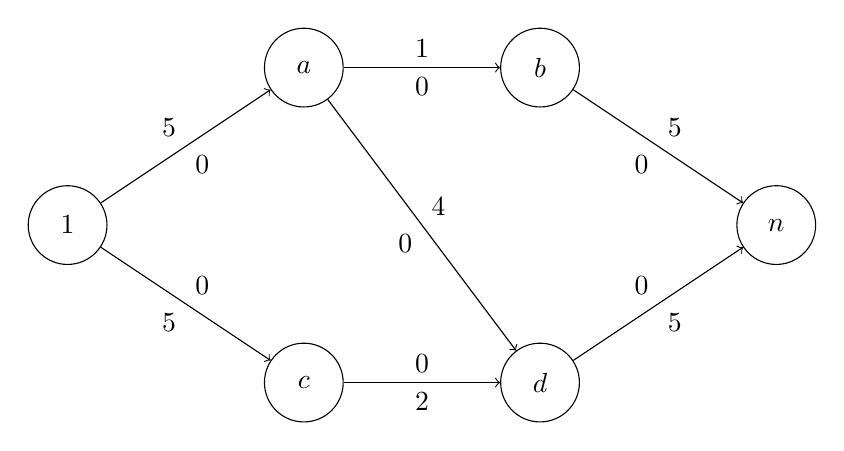
\begin{tikzpicture}[
            node distance=2cm,
            vertex/.style={
                circle,
                draw,
                minimum size=1cm,
                inner sep=0pt
            }
        ]

            \node[vertex] (1) at (0, 0) {\(1\)};
            \node[vertex] (a) at (3, 2) {\(a\)};
            \node[vertex] (c) at (3, -2) {\(c\)};
            \node[vertex] (b) at (6, 2) {\(b\)};
            \node[vertex] (d) at (6, -2) {\(d\)};
            \node[vertex] (n) at (9, 0) {\(n\)};

            \draw[->] (1) -- (a)
                node[midway, above left] {\(\boxed{5}\)}
                node[midway, below right] {\(0\)};

            \draw[->] (a) -- (b)
                node[midway, above] {\(\boxed{1}\)}
                node[midway, below] {\(0\)};

            \draw[->] (b) -- (n)
                node[midway, above right] {\(\boxed{5}\)}
                node[midway, below left] {\(0\)};

            \draw[->] (1) -- (c)
                node[midway, below left] {\(\boxed{5}\)}
                node[midway, above right] {\(0\)};

            \draw[->] (c) -- (d)
                node[midway, below] {\(\boxed{2}\)}
                node[midway, above] {\(0\)};

            \draw[->] (d) -- (n)
                node[midway, below right] {\(\boxed{5}\)}
                node[midway, above left] {\(0\)};

            \draw[->] (a) -- (d)
                node[midway, above right] {\(\boxed{4}\)}
                node[midway, below left] {\(0\)};
        \end{tikzpicture}
    \end{center}

    All the paths from \(1\) to \(n\) are:
    \begin{itemize}
        \item \(1 \to a \to b \to n\);
        \item \(1 \to a \to d \to n\);
        \item \(1 \to c \to d \to n\).
    \end{itemize}

    Augmenting the path \(1 \to a \to b \to n\), we increase the flow along this by \(1\), giving the value of the flow as \(1\):
    \begin{center}
        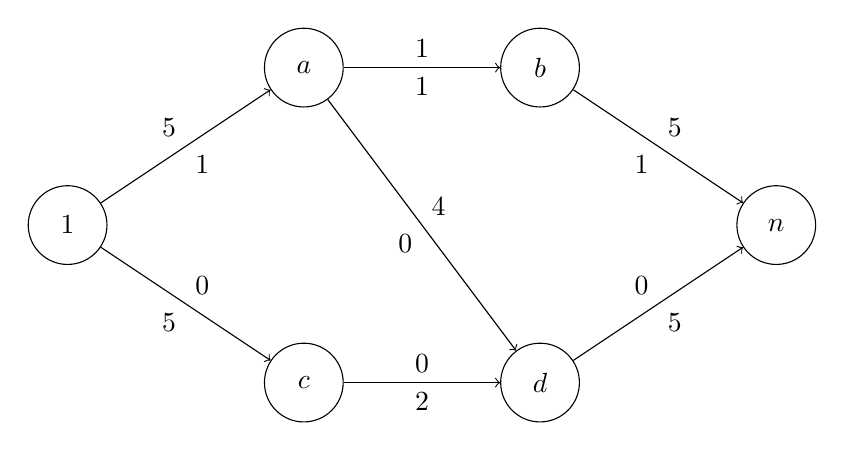
\begin{tikzpicture}[
            node distance=2cm,
            vertex/.style={
                circle,
                draw,
                minimum size=1cm,
                inner sep=0pt
            }
        ]

            \node[vertex] (1) at (0, 0) {\(1\)};
            \node[vertex] (a) at (3, 2) {\(a\)};
            \node[vertex] (c) at (3, -2) {\(c\)};
            \node[vertex] (b) at (6, 2) {\(b\)};
            \node[vertex] (d) at (6, -2) {\(d\)};
            \node[vertex] (n) at (9, 0) {\(n\)};

            \draw[->] (1) -- (a)
                node[midway, above left] {\(\boxed{5}\)}
                node[midway, below right] {\(1\)};

            \draw[->] (a) -- (b)
                node[midway, above] {\(\boxed{1}\)}
                node[midway, below] {\(1\)};

            \draw[->] (b) -- (n)
                node[midway, above right] {\(\boxed{5}\)}
                node[midway, below left] {\(1\)};

            \draw[->] (1) -- (c)
                node[midway, below left] {\(\boxed{5}\)}
                node[midway, above right] {\(0\)};

            \draw[->] (c) -- (d)
                node[midway, below] {\(\boxed{2}\)}
                node[midway, above] {\(0\)};

            \draw[->] (d) -- (n)
                node[midway, below right] {\(\boxed{5}\)}
                node[midway, above left] {\(0\)};

            \draw[->] (a) -- (d)
                node[midway, above right] {\(\boxed{4}\)}
                node[midway, below left] {\(0\)};
        \end{tikzpicture}
    \end{center}

    Augmenting the path \(1 \to a \to d \to n\), we increase the flow along this by \(4\), giving the value of the flow as \(5\):
    \begin{center}
        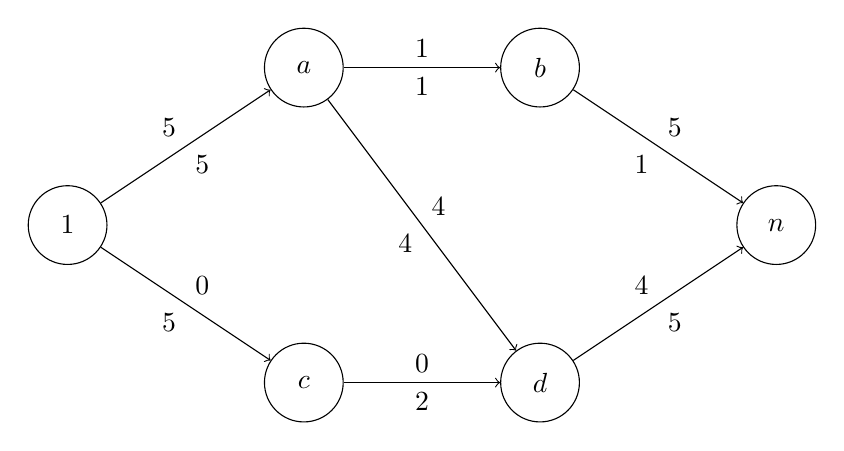
\begin{tikzpicture}[
            node distance=2cm,
            vertex/.style={
                circle,
                draw,
                minimum size=1cm,
                inner sep=0pt
            }
        ]

            \node[vertex] (1) at (0, 0) {\(1\)};
            \node[vertex] (a) at (3, 2) {\(a\)};
            \node[vertex] (c) at (3, -2) {\(c\)};
            \node[vertex] (b) at (6, 2) {\(b\)};
            \node[vertex] (d) at (6, -2) {\(d\)};
            \node[vertex] (n) at (9, 0) {\(n\)};

            \draw[->] (1) -- (a)
                node[midway, above left] {\(\boxed{5}\)}
                node[midway, below right] {\(5\)};

            \draw[->] (a) -- (b)
                node[midway, above] {\(\boxed{1}\)}
                node[midway, below] {\(1\)};

            \draw[->] (b) -- (n)
                node[midway, above right] {\(\boxed{5}\)}
                node[midway, below left] {\(1\)};

            \draw[->] (1) -- (c)
                node[midway, below left] {\(\boxed{5}\)}
                node[midway, above right] {\(0\)};

            \draw[->] (c) -- (d)
                node[midway, below] {\(\boxed{2}\)}
                node[midway, above] {\(0\)};

            \draw[->] (d) -- (n)
                node[midway, below right] {\(\boxed{5}\)}
                node[midway, above left] {\(4\)};

            \draw[->] (a) -- (d)
                node[midway, above right] {\(\boxed{4}\)}
                node[midway, below left] {\(4\)};
        \end{tikzpicture}
    \end{center}

    Augmenting the path \(1 \to b \to d \to n\), we increase the flow along this by \(1\), giving the value of the flow as \(6\):
    \begin{center}
        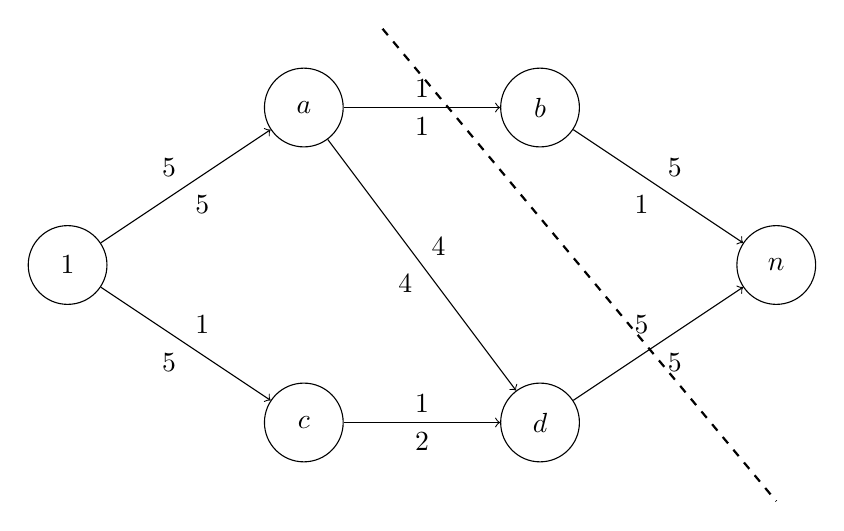
\begin{tikzpicture}[
            node distance=2cm,
            vertex/.style={
                circle,
                draw,
                minimum size=1cm,
                inner sep=0pt
            }
        ]

            \node[vertex] (1) at (0, 0) {\(1\)};
            \node[vertex] (a) at (3, 2) {\(a\)};
            \node[vertex] (c) at (3, -2) {\(c\)};
            \node[vertex] (b) at (6, 2) {\(b\)};
            \node[vertex] (d) at (6, -2) {\(d\)};
            \node[vertex] (n) at (9, 0) {\(n\)};

            \draw[->] (1) -- (a)
                node[midway, above left] {\(\boxed{5}\)}
                node[midway, below right] {\(5\)};

            \draw[->] (a) -- (b)
                node[midway, above] {\(\boxed{1}\)}
                node[midway, below] {\(1\)};

            \draw[->] (b) -- (n)
                node[midway, above right] {\(\boxed{5}\)}
                node[midway, below left] {\(1\)};

            \draw[->] (1) -- (c)
                node[midway, below left] {\(\boxed{5}\)}
                node[midway, above right] {\(1\)};

            \draw[->] (c) -- (d)
                node[midway, below] {\(\boxed{2}\)}
                node[midway, above] {\(1\)};

            \draw[->] (d) -- (n)
                node[midway, below right] {\(\boxed{5}\)}
                node[midway, above left] {\(5\)};

            \draw[->] (a) -- (d)
                node[midway, above right] {\(\boxed{4}\)}
                node[midway, below left] {\(4\)};

            \draw[dashed, thick] (4, 3) -- (9, -3);
        \end{tikzpicture}
    \end{center}

    Indeed, at this point, notice the cut \(S = \Bqty{1, a, c, d}\) satisfies \(C\pqty{S} = 6\). This is hence the maximum flow (and the corresponding minimum cut).
\end{example}

\subsubsection{The Edmonds--Karp Algorithm and Convergence of the Ford--Fulkerson Algorithm}

One unsatisfying thing about the Ford--Fulkerson algorithm is it is not very obvious how this is related to the simplex algorithm. Indeed, the Ford--Fulkerson algorithm works relatively differently, in the sense that it does not necessarily jump to extreme points -- and hence convergence is not necessarily guaranteed (thought it is guaranteed to improve). In the case where all capacities are integral (in which case all increases are also integral) or rational (in which we could just scale the problem to be integral), it is guaranteed to converge after finitely many steps.

The Edmonds--Karp algorithm which augments the path in order of distance (i.e., finding such paths by breadth-first search), guarantees for the convergence of the algorithm in \(\bigO\pqty{\abs{V} \abs{E}^2}\) time.

\begin{example}[Ford--Fulkerson Algorithm, Second Example]
    Consider the following network. (At the moment all flow is zero, and the capacities are boxed.)

    \begin{center}
        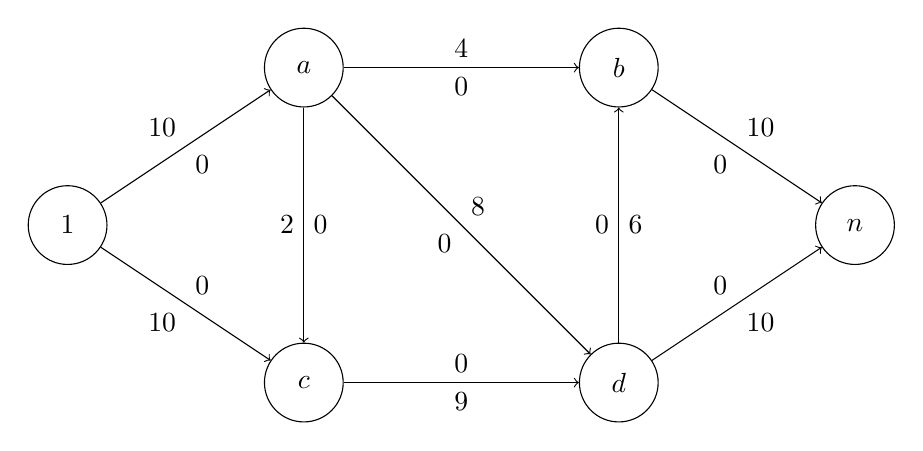
\begin{tikzpicture}[
            node distance=2cm,
            vertex/.style={
                circle,
                draw,
                minimum size=1cm,
                inner sep=0pt
            }
        ]

            \node[vertex] (1) at (0, 0) {\(1\)};
            \node[vertex] (a) at (3, 2) {\(a\)};
            \node[vertex] (c) at (3, -2) {\(c\)};
            \node[vertex] (b) at (7, 2) {\(b\)};
            \node[vertex] (d) at (7, -2) {\(d\)};
            \node[vertex] (n) at (10, 0) {\(n\)};



            \draw[->] (1) -- (a)
                node[midway, above left] {\(\boxed{10}\)}
                node[midway, below right] {\(0\)};

            \draw[->] (a) -- (b)
                node[midway, above] {\(\boxed{4}\)}
                node[midway, below] {\(0\)};

            \draw[->] (b) -- (n)
                node[midway, above right] {\(\boxed{10}\)}
                node[midway, below left] {\(0\)};

            \draw[->] (1) -- (c)
                node[midway, below left] {\(\boxed{10}\)}
                node[midway, above right] {\(0\)};

            \draw[->] (c) -- (d)
                node[midway, below] {\(\boxed{9}\)}
                node[midway, above] {\(0\)};

            \draw[->] (d) -- (n)
                node[midway, below right] {\(\boxed{10}\)}
                node[midway, above left] {\(0\)};

            \draw[->] (a) -- (c)
                node[midway, left] {\(\boxed{2}\)}
                node[midway, right] {\(0\)};

            \draw[->] (d) -- (b)
                node[midway, right] {\(\boxed{6}\)}
                node[midway, left] {\(0\)};

            \draw[->] (a) -- (d)
                node[midway, above right] {\(\boxed{8}\)}
                node[midway, below left] {\(0\)};
        \end{tikzpicture}
    \end{center}

    We find the augmenting paths. The first one would be \(1 \to a \to b \to n\), which has capacity \(4\) (increasing the value to 4), giving
    \begin{center}
        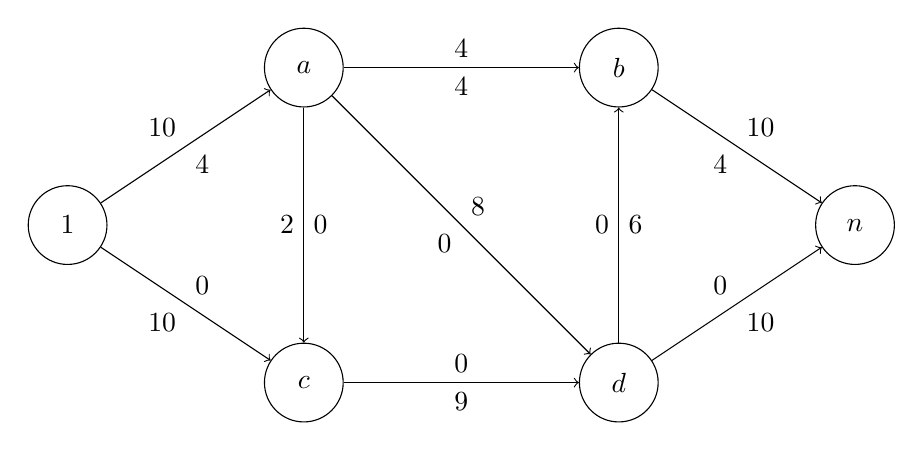
\begin{tikzpicture}[
            node distance=2cm,
            vertex/.style={
                circle,
                draw,
                minimum size=1cm,
                inner sep=0pt
            }
        ]

            \node[vertex] (1) at (0, 0) {\(1\)};
            \node[vertex] (a) at (3, 2) {\(a\)};
            \node[vertex] (c) at (3, -2) {\(c\)};
            \node[vertex] (b) at (7, 2) {\(b\)};
            \node[vertex] (d) at (7, -2) {\(d\)};
            \node[vertex] (n) at (10, 0) {\(n\)};



            \draw[->] (1) -- (a)
                node[midway, above left] {\(\boxed{10}\)}
                node[midway, below right] {\(4\)};

            \draw[->] (a) -- (b)
                node[midway, above] {\(\boxed{4}\)}
                node[midway, below] {\(4\)};

            \draw[->] (b) -- (n)
                node[midway, above right] {\(\boxed{10}\)}
                node[midway, below left] {\(4\)};

            \draw[->] (1) -- (c)
                node[midway, below left] {\(\boxed{10}\)}
                node[midway, above right] {\(0\)};

            \draw[->] (c) -- (d)
                node[midway, below] {\(\boxed{9}\)}
                node[midway, above] {\(0\)};

            \draw[->] (d) -- (n)
                node[midway, below right] {\(\boxed{10}\)}
                node[midway, above left] {\(0\)};

            \draw[->] (a) -- (c)
                node[midway, left] {\(\boxed{2}\)}
                node[midway, right] {\(0\)};

            \draw[->] (d) -- (b)
                node[midway, right] {\(\boxed{6}\)}
                node[midway, left] {\(0\)};

            \draw[->] (a) -- (d)
                node[midway, above right] {\(\boxed{8}\)}
                node[midway, below left] {\(0\)};
        \end{tikzpicture}
    \end{center}

    We look at \(1 \to a \to d \to n\), which has a capacity of \(6\) (increasing the value to 10), giving
    \begin{center}
        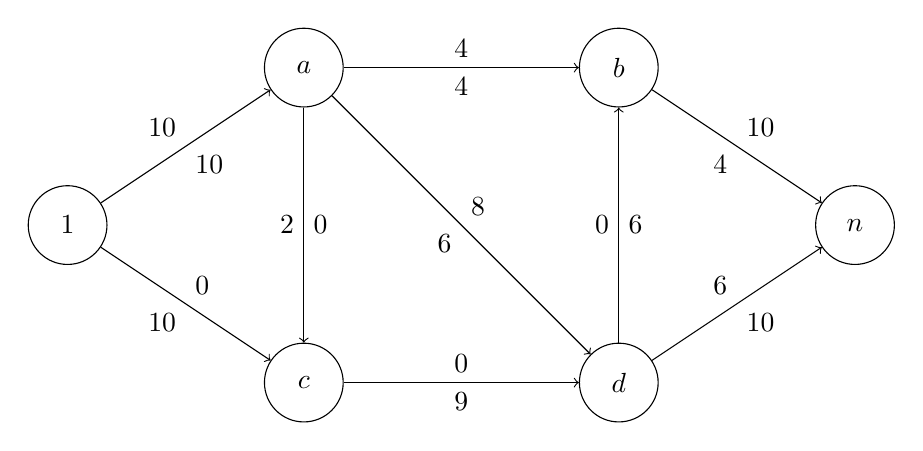
\begin{tikzpicture}[
            node distance=2cm,
            vertex/.style={
                circle,
                draw,
                minimum size=1cm,
                inner sep=0pt
            }
        ]

            \node[vertex] (1) at (0, 0) {\(1\)};
            \node[vertex] (a) at (3, 2) {\(a\)};
            \node[vertex] (c) at (3, -2) {\(c\)};
            \node[vertex] (b) at (7, 2) {\(b\)};
            \node[vertex] (d) at (7, -2) {\(d\)};
            \node[vertex] (n) at (10, 0) {\(n\)};



            \draw[->] (1) -- (a)
                node[midway, above left] {\(\boxed{10}\)}
                node[midway, below right] {\(10\)};

            \draw[->] (a) -- (b)
                node[midway, above] {\(\boxed{4}\)}
                node[midway, below] {\(4\)};

            \draw[->] (b) -- (n)
                node[midway, above right] {\(\boxed{10}\)}
                node[midway, below left] {\(4\)};

            \draw[->] (1) -- (c)
                node[midway, below left] {\(\boxed{10}\)}
                node[midway, above right] {\(0\)};

            \draw[->] (c) -- (d)
                node[midway, below] {\(\boxed{9}\)}
                node[midway, above] {\(0\)};

            \draw[->] (d) -- (n)
                node[midway, below right] {\(\boxed{10}\)}
                node[midway, above left] {\(6\)};

            \draw[->] (a) -- (c)
                node[midway, left] {\(\boxed{2}\)}
                node[midway, right] {\(0\)};

            \draw[->] (d) -- (b)
                node[midway, right] {\(\boxed{6}\)}
                node[midway, left] {\(0\)};

            \draw[->] (a) -- (d)
                node[midway, above right] {\(\boxed{8}\)}
                node[midway, below left] {\(6\)};
        \end{tikzpicture}
    \end{center}

    The next one would be \(1 \to c \to d \to n\), with a capacity of \(4\) (increasing the value to 14), giving
    \begin{center}
        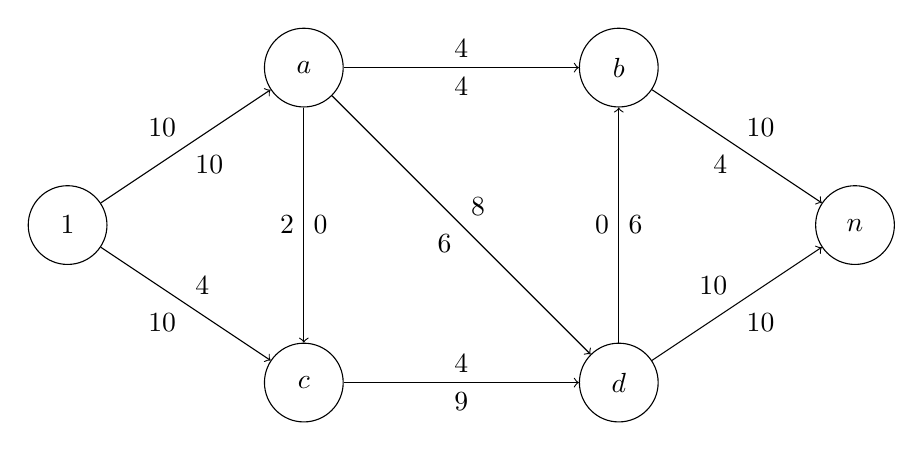
\begin{tikzpicture}[
            node distance=2cm,
            vertex/.style={
                circle,
                draw,
                minimum size=1cm,
                inner sep=0pt
            }
        ]

            \node[vertex] (1) at (0, 0) {\(1\)};
            \node[vertex] (a) at (3, 2) {\(a\)};
            \node[vertex] (c) at (3, -2) {\(c\)};
            \node[vertex] (b) at (7, 2) {\(b\)};
            \node[vertex] (d) at (7, -2) {\(d\)};
            \node[vertex] (n) at (10, 0) {\(n\)};



            \draw[->] (1) -- (a)
                node[midway, above left] {\(\boxed{10}\)}
                node[midway, below right] {\(10\)};

            \draw[->] (a) -- (b)
                node[midway, above] {\(\boxed{4}\)}
                node[midway, below] {\(4\)};

            \draw[->] (b) -- (n)
                node[midway, above right] {\(\boxed{10}\)}
                node[midway, below left] {\(4\)};

            \draw[->] (1) -- (c)
                node[midway, below left] {\(\boxed{10}\)}
                node[midway, above right] {\(4\)};

            \draw[->] (c) -- (d)
                node[midway, below] {\(\boxed{9}\)}
                node[midway, above] {\(4\)};

            \draw[->] (d) -- (n)
                node[midway, below right] {\(\boxed{10}\)}
                node[midway, above left] {\(10\)};

            \draw[->] (a) -- (c)
                node[midway, left] {\(\boxed{2}\)}
                node[midway, right] {\(0\)};

            \draw[->] (d) -- (b)
                node[midway, right] {\(\boxed{6}\)}
                node[midway, left] {\(0\)};

            \draw[->] (a) -- (d)
                node[midway, above right] {\(\boxed{8}\)}
                node[midway, below left] {\(6\)};
        \end{tikzpicture}
    \end{center}

    All paths of length 3 has been augmented, and therefore we look at paths of length 4. Augmenting the path \(1 \to c \to d \to b \to n\) increases the capacity by \(5\) (increasing the value to \(19\)), which gives
    \begin{center}
        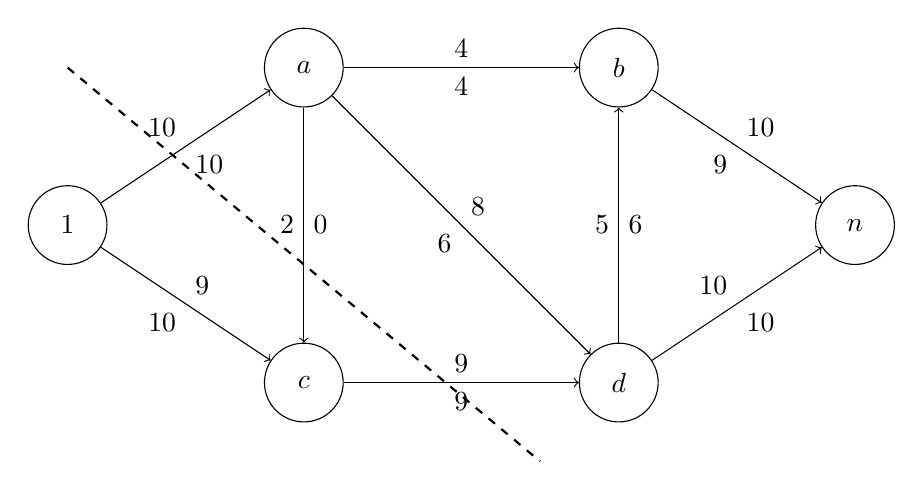
\begin{tikzpicture}[
            node distance=2cm,
            vertex/.style={
                circle,
                draw,
                minimum size=1cm,
                inner sep=0pt
            }
        ]

            \node[vertex] (1) at (0, 0) {\(1\)};
            \node[vertex] (a) at (3, 2) {\(a\)};
            \node[vertex] (c) at (3, -2) {\(c\)};
            \node[vertex] (b) at (7, 2) {\(b\)};
            \node[vertex] (d) at (7, -2) {\(d\)};
            \node[vertex] (n) at (10, 0) {\(n\)};



            \draw[->] (1) -- (a)
                node[midway, above left] {\(\boxed{10}\)}
                node[midway, below right] {\(10\)};

            \draw[->] (a) -- (b)
                node[midway, above] {\(\boxed{4}\)}
                node[midway, below] {\(4\)};

            \draw[->] (b) -- (n)
                node[midway, above right] {\(\boxed{10}\)}
                node[midway, below left] {\(9\)};

            \draw[->] (1) -- (c)
                node[midway, below left] {\(\boxed{10}\)}
                node[midway, above right] {\(9\)};

            \draw[->] (c) -- (d)
                node[midway, below] {\(\boxed{9}\)}
                node[midway, above] {\(9\)};

            \draw[->] (d) -- (n)
                node[midway, below right] {\(\boxed{10}\)}
                node[midway, above left] {\(10\)};

            \draw[->] (a) -- (c)
                node[midway, left] {\(\boxed{2}\)}
                node[midway, right] {\(0\)};

            \draw[->] (d) -- (b)
                node[midway, right] {\(\boxed{6}\)}
                node[midway, left] {\(5\)};

            \draw[->] (a) -- (d)
                node[midway, above right] {\(\boxed{8}\)}
                node[midway, below left] {\(6\)};

            \draw[dashed, thick] (0, 2) -- (6, -3);
        \end{tikzpicture}
    \end{center}

    Indeed, notice the cut \(S = \Bqty{1, c}\) gives a cut of \(19\), and hence this must be optimal.
\end{example}

\subsubsection{Duality of Maximum Flow and Minimum Cut}

We have discussed a lot about duality of problems in this course, and it is very tempting to prove that maximum flow corresponding to minimum cut is a duality problem. (This is also suggested by our two-part theorem proof.) However, it is not immediately clear how minimum cut can be a linear programming problem.

Recall the notation
\[
    b_i = \begin{cases}
        +1, &\qif i = 1, \\
        -1, &\qif i = n, \\
        0, &\qotherwise.
    \end{cases}
\]
and the primal becomes maximising \(\delta\), subject to
\[
    \sum_{j: \pqty{i, j} \in E} x_{ij} - \sum_{j: \pqty{j, i} \in E} x_{ji} = b_i \delta.
\]
and
\[
    0 \leq x_{ij} \leq c_{ij}.
\]

We introduce dual variables \(y_i\) for each vertex \(i\) for the equality constraints, and introduce slack variables \(s_{ij} \geq 0\) for each edge with corresponding dual variables \(z_{ij}\). Then, the Lagrangian of the primal problem is therefore (since \(\delta\) is to be maximised)
\begin{align*}
    L\pqty{\delta, \pqty{x_{ij}}, \pqty{s_{ij}}, \pqty{y_i}, \pqty{z_{ij}}} &= \pqty{-\delta} - \sum_{i \in V} y_i \pqty{\phi_i \pqty{x} - b_i \delta} - \sum_{\pqty{i, j} \in E} z_{ij} \pqty{c_{ij} - x_{ij} - s_{ij}} \\
    &= \pqty{-1 + \sum_{i \in V} y_i b_i} \delta - \sum_{i \in V} y_i \pqty{\sum_{j: \pqty{i, j} \in E} x_{ij} - \sum_{j: \pqty{j, i} \in E} x_{ji}} \\
    &\phantom{=} \hspace{5em} - \sum_{\pqty{i, j} \in E} z_{ij} c_{ij} + \sum_{\pqty{i, j} \in E} z_{ij} x_{ij} + \sum_{\pqty{i, j} \in E} z_{ij} s_{ij} \\
    &= \pqty{-1 + \sum_{i \in V} y_i b_i} \delta - \sum_{\pqty{i, j} \in E} y_i x_{ij} + \sum_{\pqty{j, i} \in E} y_i x_{ji} \\
    &\phantom{=} \hspace{5em} - \sum_{\pqty{i, j} \in E} z_{ij} c_{ij} + \sum_{\pqty{i, j} \in E} z_{ij} x_{ij} + \sum_{\pqty{i, j} \in E} z_{ij} s_{ij} \\
    &=  \pqty{-1 + \sum_{i \in V} y_i b_i} \delta + \sum_{\pqty{i, j} \in E} \pqty{- y_i + y_j + z_{ij}} x_{ij} \\
    &\phantom{=} \hspace{12em} + \sum_{\pqty{i, j} \in E} z_{ij} s_{ij} - \sum_{\pqty{i, j} \in E} z_{ij} c_{ij}.
\end{align*}

Therefore, the dual feasible set is given by
\[
    \sum_{i \in V} y_i b_i = 1 \qand z_{ij} \geq y_i - y_j \qand z_{ij} \geq 0.
\]

Notice the first constraint reduces to
\[
    y_1 - y_n = 1
\]
where \(1\) is the source vertex and \(n\) is the sink vertex. With this, the dual function is given by
\[
    -\sum_{\pqty{i, j} \in E} z_{ij} c_{ij}
\]
and the dual problem is, hence, to minimise
\[
    \sum_{\pqty{i, j} \in E} z_{ij} c_{ij}
\]
subject to constraints
\begin{align*}
    y_1 - y_n &= 1 \\
    z_{ij} &\geq y_i - y_j \\
    z_{ij} &\geq 0.
\end{align*}

Notice that to minimise this, since all the capacities are non-negative, we always take
\[
    z_{ij} = \max \Bqty{0, y_i - y_j}
\]
and the dual objective is now minimising
\[
    \sum_{\pqty{i, j} \in E} \max \Bqty{0, y_i - y_j} c_{ij}
\]
subject to \(y_1 - y_n = 1\).

To note this relation with the minimum cut problem, note that a cut \(\pqty{S, V \setminus S}\) assigned with \(y_i = 1\) for \(i \in S\) and \(0\) for \(i \in V \setminus S\), we have the constraint translates to \(1 \in S\) and \(n \in V \setminus S\), and
\[
    \sum_{\pqty{i, j} \in E} \max \Bqty{0, y_i - y_j} c_{ij} = \sum_{\substack{\pqty{i, j} \in E \\ i \in S \\ j \in V \setminus S}} c_{ij} = C\pqty{S}
\]
is indeed the capacity, so the minimum of the dual objective function is at most the minimum cut. With some more technical details, we can indeed show any \(y_i\)s that minimises of this dual objective function can be \(\Bqty{0, 1}\), fully leading to the equivalence.